\section{重参数化估计}
\label{sec:pgrad-reparam}

回到章首的问题：$X\sim\mathcal{N}(\theta,1)$，$J(\theta)=\mathbb{E}[X^{2}]$。参数改变的是分布，上一节的方法不能直接用。但第~\ref{chap:sample-generation}章的生成方法提示了另一种写法：先抽$\varepsilon\sim\mathcal{N}(0,1)$，再令$X=\theta+\varepsilon$。噪声的分布与$\theta$无关，参数只出现在这个确定的映射里，于是分布的变化被改写成了函数的变化。

\paragraph{生成映射与梯度表示}

一般地，设噪声$\varepsilon$取值于某个空间、分布为$Q$且不依赖参数，$T_{\bm{\theta}}$是从噪声到$\mathbb{R}^{d}$的映射，使$T_{\bm{\theta}}(\varepsilon)$的分布正是$P_{\bm{\theta}}$，即$P_{\bm{\theta}}$是$Q$在$T_{\bm{\theta}}$下的推前。这样的写法称为\term{重参数化}（reparameterization）。由推前的换元公式，
\begin{equation}
  J(\bm{\theta})=\mathbb{E}_{Q}\bigl[f_{\bm{\theta}}(T_{\bm{\theta}}(\varepsilon))\bigr].
  \label{eq:pgrad-reparam-J}
\end{equation}
期望所对的分布$Q$固定，形式上回到了上一节：在定理~\ref{thm:pgrad-exchange}中取$\mu=Q$，以式~\eqref{eq:pgrad-reparam-J}方括号内的复合函数作$g(\bm{\theta},\varepsilon)$即可。

对固定的$\varepsilon$求$g$对$\bm{\theta}$的导数，要用链式法则。设$f_{\bm{\theta}}(x)$对$(\bm{\theta},x)$连续可微，$T_{\bm{\theta}}(\varepsilon)$对$\bm{\theta}$可微，记$x=T_{\bm{\theta}}(\varepsilon)$，$D_{\bm{\theta}}T_{\bm{\theta}}(\varepsilon)$为$d\times k$的Jacobi矩阵。参数沿两条路到达函数值：一条直接进入$f_{\bm{\theta}}$，另一条先移动样本点$x$，再经$f_{\bm{\theta}}$对$x$的梯度传到函数值。两条路的贡献相加，
\begin{equation}
  \nabla_{\bm{\theta}}\bigl[f_{\bm{\theta}}(T_{\bm{\theta}}(\varepsilon))\bigr]
  =\nabla_{\bm{\theta}}f_{\bm{\theta}}(x)+\bigl(D_{\bm{\theta}}T_{\bm{\theta}}(\varepsilon)\bigr)^{\top}\nabla_{x}f_{\bm{\theta}}(x).
  \label{eq:pgrad-chain}
\end{equation}
图~\ref{fig:pgrad-chain-paths}画出这两条路。称它为沿样本生成路径的导数，即\term{路径导数}（pathwise derivative）。

\begin{BookInlineFigure}
  \centering
  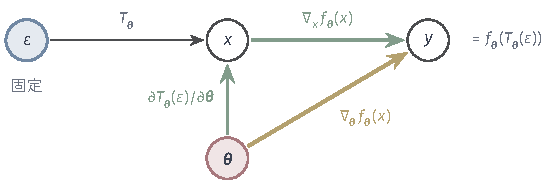
\includegraphics[width=94mm]{figures/07-probability/08-sampling-and-integration/tikz/pgrad-chain-paths/figure.pdf}
  \caption{一个重参数化样本的计算图。噪声$\varepsilon$（蓝）固定，参数$\bm{\theta}$（红）经两条路影响函数值$y$：黄色箭头是函数自身对参数的导数，绿色箭头是先经生成映射移动样本点、再经函数对$x$的梯度传递的部分。路径导数是两部分之和。}
  \label{fig:pgrad-chain-paths}
\end{BookInlineFigure}

把这些条件合起来，就得到重参数化的梯度表示。

\begin{theorem}[重参数化梯度]
\label{thm:pgrad-reparam}
设$P_{\bm{\theta}}$是$Q$在$T_{\bm{\theta}}$下的推前，$U$是以$\bm{\theta}_{0}$为中心的开球，复合函数$g(\bm{\theta},\varepsilon)$等于$f_{\bm{\theta}}(T_{\bm{\theta}}(\varepsilon))$。设对$Q$几乎所有$\varepsilon$，$\bm{\theta}\mapsto T_{\bm{\theta}}(\varepsilon)$在$\bm{\theta}_{0}$处可微，$(\bm{\theta},x)\mapsto f_{\bm{\theta}}(x)$在$(\bm{\theta}_{0},T_{\bm{\theta}_{0}}(\varepsilon))$的某个邻域内连续可微；又设$g$满足定理~\ref{thm:pgrad-exchange}的条件1与条件3（取$\mu=Q$）。记$X=T_{\bm{\theta}_{0}}(\varepsilon)$，则
\begin{equation}
  \nabla J(\bm{\theta}_{0})=\mathbb{E}_{Q}\Bigl[\nabla_{\bm{\theta}}f_{\bm{\theta}_{0}}(X)+\bigl(D_{\bm{\theta}}T_{\bm{\theta}_{0}}(\varepsilon)\bigr)^{\top}\nabla_{x}f_{\bm{\theta}_{0}}(X)\Bigr].
  \label{eq:pgrad-reparam}
\end{equation}
\end{theorem}

证明就是定理~\ref{thm:pgrad-exchange}本身。所设的可微性使链式法则对几乎所有$\varepsilon$成立，于是$g(\cdot,\varepsilon)$在$\bm{\theta}_{0}$处可微，梯度由式~\eqref{eq:pgrad-chain}给出，这正是定理~\ref{thm:pgrad-exchange}的条件2；再由式~\eqref{eq:pgrad-exchange}，$J$的梯度等于这些逐点梯度关于$Q$的积分。对独立的$\varepsilon_{1},\dots,\varepsilon_{n}\sim Q$，令$X_{i}=T_{\bm{\theta}}(\varepsilon_{i})$，\term{重参数化估计}（reparameterization gradient estimator）是式~\eqref{eq:pgrad-reparam}方括号内的量在这$n$个样本上的平均，记作$\hat{\bm{g}}_{n}^{\mathrm{rep}}$。无偏性、一致性与均方误差的讨论与上一节完全相同。

\paragraph{高斯的平移与尺度}

最常用的生成映射是高斯的位置尺度变换$X=\mu+\sigma\varepsilon$，$\varepsilon\sim\mathcal{N}(0,1)$，参数$\bm{\theta}=(\mu,\sigma)$，$\sigma>0$。映射对参数的导数是
\[
  \frac{\partial X}{\partial\mu}=1,\qquad\frac{\partial X}{\partial\sigma}=\varepsilon .
\]
增大$\mu$时每个样本平移同样的距离；增大$\sigma$时每个样本沿远离$\mu$的方向移动，移动量与它的$\varepsilon$成正比，$\varepsilon$为负的样本向左走，为正的向右走。图~\ref{fig:pgrad-reparam-map}用四个固定的$\varepsilon$画出了这两种移动。

\begin{BookInlineFigure}
  \centering
  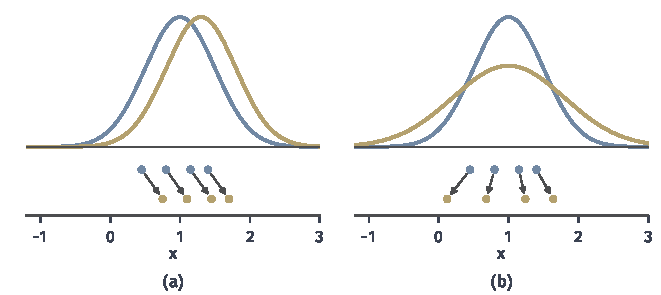
\includegraphics[width=112mm]{figures/07-probability/08-sampling-and-integration/matplotlib/pgrad-reparam-map/figure.pdf}
  \caption{高斯位置尺度变换下同一组噪声$\varepsilon=0.3,-1.1,0.8,-0.4$的样本怎样移动。蓝线与蓝点为$(\mu,\sigma)=(1,0.5)$时的密度与样本，黄线与黄点为参数改变后的密度与样本，箭头连接同一个$\varepsilon$生成的两个样本。(a)$\mu$由$1$变为$1.3$，各样本平移$0.3$；(b)$\sigma$由$0.5$变为$0.8$，样本$i$移动$0.3\varepsilon_{i}$。}
  \label{fig:pgrad-reparam-map}
\end{BookInlineFigure}

取$f(x)=x^{2}$，$J(\mu,\sigma)=\mu^{2}+\sigma^{2}$，梯度是$(2\mu,2\sigma)$。函数不含参数，式~\eqref{eq:pgrad-chain}只剩生成映射一项，两个分量的路径导数分别为
\[
  G_{\mu}=2X,\qquad G_{\sigma}=2X\varepsilon .
\]
由$\mathbb{E}[\varepsilon]=0$与$\mathbb{E}[\varepsilon^{2}]=1$，它们的期望是
\[
  \mathbb{E}[2X]=2\mu,\qquad\mathbb{E}[2(\mu+\sigma\varepsilon)\varepsilon]=2\sigma,
\]
与真值一致。交换条件也容易验证：参数限制在$\lvert\mu'-\mu\rvert<\delta$、$\lvert\sigma'-\sigma\rvert<\delta$内时，
\[
  \lvert G_{\mu}\rvert+\lvert G_{\sigma}\rvert\leq2\bigl(\lvert\mu\rvert+\delta+(\sigma+\delta)\lvert\varepsilon\rvert\bigr)(1+\lvert\varepsilon\rvert),
\]
右边是$\lvert\varepsilon\rvert$的二次多项式，在标准正态下可积。

下面用固定的噪声手算一次。取$(\mu,\sigma)=(1,0.5)$与$\varepsilon=0.3,-1.1,0.8,-0.4$，样本是
\[
  X=1.15,\ 0.45,\ 1.40,\ 0.80 .
\]
$\mu$分量的四个路径导数及其平均为
\[
  G_{\mu}=2.30,\ 0.90,\ 2.80,\ 1.60,\qquad\hat{g}_{\mu}=1.900,
\]
真值是$2$。$\sigma$分量为
\[
  G_{\sigma}=0.69,\ -0.99,\ 2.24,\ -0.64,\qquad\hat{g}_{\sigma}=0.325,
\]
真值是$1$。

$\sigma$分量偏得多，这不是计算错误。两个分量的单样本方差是
\[
  \operatorname{Var}(2X)=4\sigma^{2}=1,\qquad\operatorname{Var}(2X\varepsilon)=\operatorname{Var}(2\mu\varepsilon+2\sigma\varepsilon^{2})=4\mu^{2}+8\sigma^{2}=6,
\]
其中用到$\varepsilon$与$\varepsilon^{2}$的协方差$\mathbb{E}[\varepsilon^{3}]$为零，以及$\operatorname{Var}(\varepsilon^{2})=2$。四样本平均下$\sigma$分量的标准差约为$\sqrt{6/4}\approx1.22$，偏离$0.675$完全正常。同一个估计的不同分量，精度可以差很多。

\paragraph{函数自身与生成映射的贡献}

当函数也含参数时，式~\eqref{eq:pgrad-chain}的两项都出现。回到第~\ref{sec:pgrad-parametric}节的例子：$X=\theta+\varepsilon$，$f_{\theta}(x)=x^{2}-\theta x$。两条路的贡献分别是
\[
  \partial_{\theta}f_{\theta}(x)=-x,\qquad\partial_{x}f_{\theta}(x)\cdot\partial_{\theta}X=(2x-\theta)\cdot1 .
\]
两者相加，
\[
  \frac{\mathrm{d}}{\mathrm{d}\theta}f_{\theta}(\theta+\varepsilon)=-X+(2X-\theta)=X-\theta=\varepsilon,
\]
期望为零，与$J(\theta)=1$一致。单独取第一项得到$\mathbb{E}[-X]=-\theta$，单独取第二项得到$\mathbb{E}[2X-\theta]=\theta$，正是图~\ref{fig:pgrad-two-terms}中黄线与紫线的斜率。重参数化把“分布的变化”具体化成了“样本点的移动”，两项各有清楚的来源。

\paragraph{离散选择与不连续的生成步骤}

重参数化要求对每个固定的噪声，函数值随参数连续地、可控地变化。离散选择破坏了这一点。设$X\sim\operatorname{Bern}(\theta)$，用逆变换写成$X=\mathbf{1}_{\{U\leq\theta\}}$，$U\sim\operatorname{Unif}(0,1)$。对任意函数$f$，
\[
  J(\theta)=\theta f(1)+(1-\theta)f(0),\qquad J'(\theta)=f(1)-f(0).
\]
但对每个$U\neq\theta$，$X$在$\theta$附近是常数，路径导数为零，平均起来还是零。

图~\ref{fig:pgrad-bernoulli-threshold}说明了导数藏在哪里。参数从$\theta$增加到$\theta+h$时，只有落在$(\theta,\theta+h]$里的$U$使$X$由$0$跳到$1$，这件事的概率是$h$，每次跳跃使函数值改变$f(1)-f(0)$。期望的变化$h\bigl(f(1)-f(0)\bigr)$全部来自这些跳跃，而对任何固定的$U$，跳跃只发生在一个参数值上，逐点求导看不到它。用定理~\ref{thm:pgrad-exchange}的语言说，$g(\theta,u)=f(\mathbf{1}_{\{u\leq\theta\}})$在$\theta$的任何邻域内都有跳跃的$u$构成正概率集合，式~\eqref{eq:pgrad-lipschitz}不可能成立。

\begin{BookInlineFigure}
  \centering
  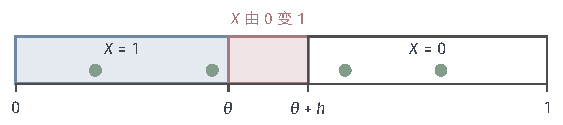
\includegraphics[width=96mm]{figures/07-probability/08-sampling-and-integration/tikz/pgrad-bernoulli-threshold/figure.pdf}
  \caption{用$X=\mathbf{1}_{\{U\leq\theta\}}$生成$\operatorname{Bern}(\theta)$。横轴是$U$的取值；蓝色区间上$X=1$。参数由$\theta=0.4$增至$\theta+h=0.55$时，只有红色区间内的$U$使$X$由$0$变为$1$，其概率为$h$。绿点是四个固定均匀数$0.37,0.80,0.15,0.62$，都不在红色区间内，它们生成的样本对参数的路径导数都是零。}
  \label{fig:pgrad-bernoulli-threshold}
\end{BookInlineFigure}

连续分布配上不连续的函数也会出同样的问题。取$f(x)=\mathbf{1}_{\{x>0\}}$，$X=\theta+\varepsilon$，则
\[
  J(\theta)=\mathbb{P}(\varepsilon>-\theta)=\Phi(\theta),\qquad J'(\theta)=\varphi(\theta)>0 .
\]对每个$\varepsilon\neq-\theta$，$f(\theta+\varepsilon)$在$\theta$附近是常数，路径导数为零。图~\ref{fig:pgrad-step-path}(a)中，四个固定噪声对应的平均$\frac{1}{4}\sum_{i}\mathbf{1}_{\{\theta+\varepsilon_{i}>0\}}$是一条阶梯，它逐段水平，导数只在台阶处“集中”。普通链式法则在这里不能直接沿用。

\begin{BookInlineFigure}
  \centering
  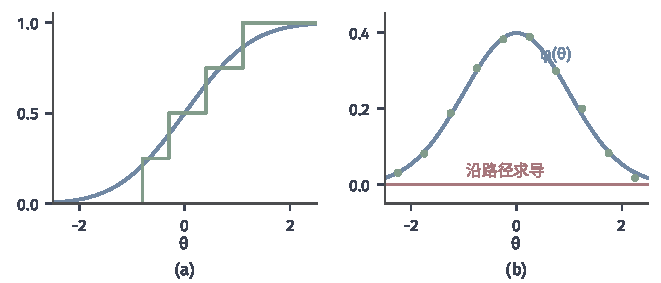
\includegraphics[width=112mm]{figures/07-probability/08-sampling-and-integration/matplotlib/pgrad-step-path/figure.pdf}
  \caption{$f(x)=\mathbf{1}_{\{x>0\}}$，$X=\theta+\varepsilon$。(a)蓝线为$J(\theta)=\Phi(\theta)$，绿色阶梯为四个固定噪声$\varepsilon=0.3,-1.1,0.8,-0.4$给出的样本平均，逐段水平。(b)蓝线为$J'(\theta)=\varphi(\theta)$，红线为路径导数的平均$0$，绿点为下一节得分函数估计在各$\theta$处的平均（每点$20000$个固定种子样本）。}
  \label{fig:pgrad-step-path}
\end{BookInlineFigure}

处理这类问题有三条出路。第一条是不对函数求导，改为对概率权重求导，这就是下一节的得分函数估计，图~\ref{fig:pgrad-step-path}(b)的绿点显示它在这个例子里给出正确的导数。第二条是把跳跃的贡献单独算出来：上例中$\frac{\mathrm{d}}{\mathrm{d}\theta}\mathbb{P}(\varepsilon>-\theta)$等于边界$\varepsilon=-\theta$处的密度，这一项可以解析地加回去。第三条是用光滑函数近似跳跃，再对近似求路径导数；这样得到的是近似问题的梯度，与原梯度的差需要另外控制。无论哪一条，都要先承认路径导数在这里不是原梯度的无偏估计。

不连续不等于不可用。若$f$是Lipschitz函数，例如$f(x)=\lvert x\rvert$，则由三角不等式
\[
  \bigl\lvert f(\theta+\varepsilon)-f(\theta'+\varepsilon)\bigr\rvert\leq\lvert\theta-\theta'\rvert,
\]
式~\eqref{eq:pgrad-lipschitz}以$M\equiv1$成立；不可微点$\theta+\varepsilon=0$只对一个$\varepsilon$出现，概率为零。于是路径导数$\operatorname{sign}(X)$的期望就是$J'(\theta)$。区分的标准不是“处处可微”，而是函数值随参数的变化能否被一个可积的Lipschitz常数控制。
